% Chapter Template

\chapter{Background} % Main chapter title

\label{chp:background} % Change X to a consecutive number; for referencing this chapter elsewhere, use~\ref{ChapterX}

This chapter includes required background to understand the thesis proposal presented in the following chapters.

\section{Convolutional Neural Networks (CNN)}
CNN is initially introduced by LeCun \cite{lecun1989handwritten} which is based on learning adaptive convolutional kernels. CNN consist of two parts convbase and densebase parts. For the Convbase instead of connecting all of the units in a layer to all the units in a preceding layer, convolutional networks organize each layer into feature maps \cite{lecun1989handwritten}, which
can be though of as parallel planes or channels. In a convolutional layer, the weighted sums are only performed within a small local window \textit{i.e)} receptive field, and weights are identical for all pixels, just as in regular shift-invariant image convolution and correlation. This parameter sharing reduce the required total number of parameter and allows learning shift invariant convolutional kernels. These convolutional kernels produce equivariant features maps. Fig.~\ref{lenet} represents typical CNN architecture of LeNet.
\begin{figure}
    \begin{center}
        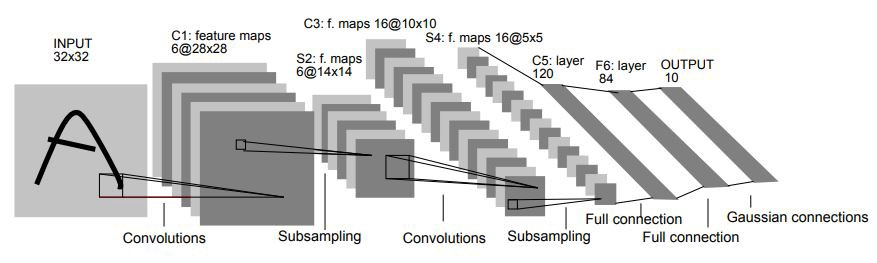
\includegraphics[width=\textwidth]{Figures/LeNetCNN.jpeg}
        \caption{Typical CNN architecture}
        \label{lenet}
    \end{center}
\end{figure}
\subsection{Convolutional Layer}
The building block of the convolutional layer is the 2D convolutional kernel. Fig.~\ref{conv2Dlayer} illustrates the 2D convolutional layer. Each 2D convolution kernel takes as input all of the $C_{i-1}$ channels in the preceding layer, windowed to a small area, and produces the values in one of the $C_{i}$ channels in the next layer. For each of the output channels, we have $K^2\times C_{i-1}$ kernel weights, so the total number of learnable parameters in each convolutional layer is $K^2\times C_{i-1} \times C_{i}$. In Fig.~\ref{conv2Dlayer}, we have $C_{i-1} = 6$ input channels and $C_{i} = 4$ output channels, with an $K = 3$ convolution window, for a total of $9 \times 6 \times 4$ learnable weights, shown in the middle column of the figure. Since the convolution is applied at each of the $W \times H$ pixels in a given layer, the amount of computation (multiply-adds) in each forward and backward pass
over one sample in a given layer is $W\times H \times K^{2} \times C_{i-1} \times C_{i}$.
To fully determine the behavior of a convolutional layer, we still need to specify the following hyperparameter:
\begin{itemize}
    \item \textbf{Padding.} Padding is used to preserve the spatial dimension of the input feature map after the convolution operation is performed. Typically, it is performed by inserting $\lfloor K/2 \rfloor$ columns for both sides and $\lfloor K/2 \rfloor$ rows to the top and bottom.
    \item \textbf{Stride.} Stride is the step taken between two centers when performing the convolution operation. Typically, Stride is equal to $1$. Stride can act as down sampling operation that can be performed instead of the pooling operation.
    \item \textbf{Dilation.} Dilation is a technique that enlarge the kernel by inserting zeros between its consecutive elements. As a result it covers a larger area of the input without increasing the total number of parameters. Which can be discribed as \[y[i]=\sum_{k}^{K} x[i+r\times k] w[k]\] where $x$ is the input signal, $w$ is the convolutional filter with size of $K$, $y$ is the resultant signal, and $r$ is the dilation rate.
\end{itemize}

\begin{figure}
    \begin{center}
        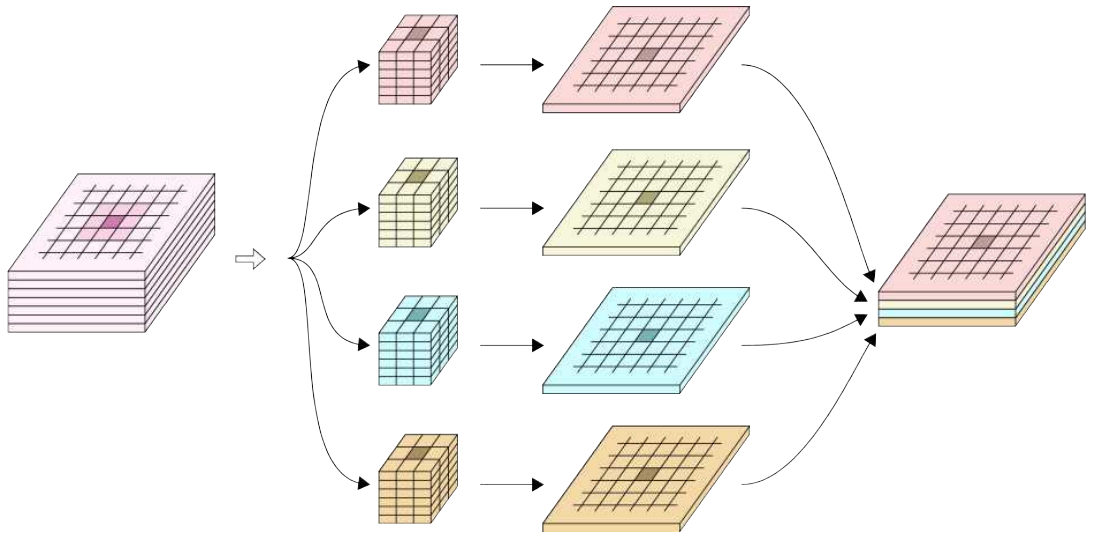
\includegraphics[width=\textwidth]{Figures/2DConvKernels.png}
        \caption{Convolutional layer with single input feature map and four convolutional kernels}
        \label{conv2Dlayer}
    \end{center}
\end{figure}


Generally, each convolutional layer computes some activation based on its input and a nonlinear function. Activation function used in each layer have a great effect on the modeling of the problem and also the semantic assigned to the output of some units is affected by this choice. The most important activation functions will be introduced in the following section.

\section{Activation functions}\label{sec:activations}
\begin{figure}
\centering
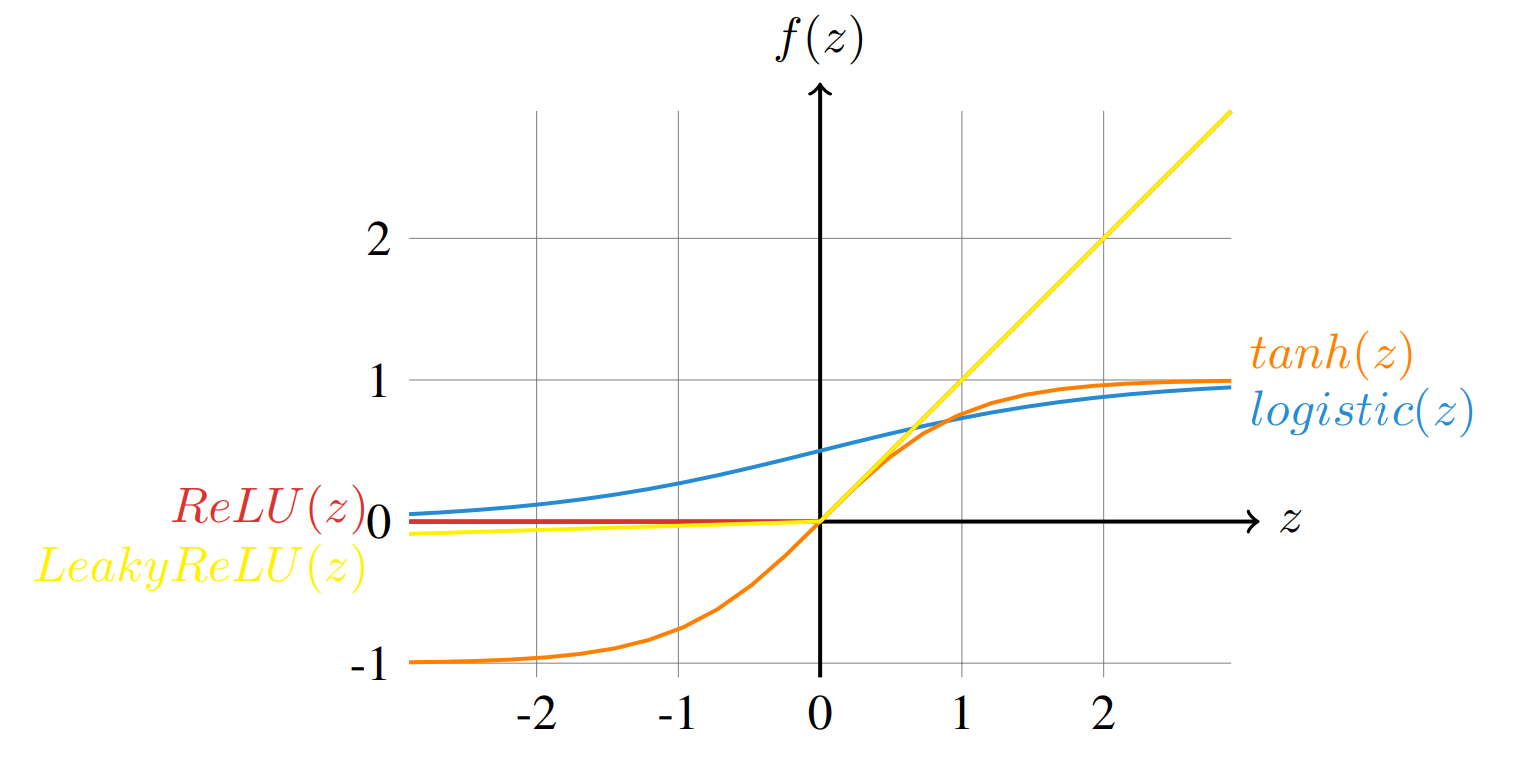
\includegraphics[width=\textwidth]{Figures/Actfuncs.png}
\caption{Some of the most common activation functions: sigmoid, tanh, ReLU and Leaky ReLU. ReLU and Leaky ReLU are overlapping for $z \geq 0$. Best viewed in colors.}
\label{fig:activations}
\end{figure}

The activation function is one of the most important component of an CNN. To tackle non-linearly separable problems it is imperative to map the input into a space that is linearly separable. The activation function does this by performing an \emph{element-wise nonlinear transformation} of the pre-activation that comes from the linear combination of the convolutional layer.

The linear combination of the convolutional layer and the nonlinearity work together closely: the latter is usually fixed and does not evolve during training, but maps its input to a highly non-linear space; the former, is determined by the learned weights which is learned during the training process and uses the activation function to map the calculated activation into a new space where they are simpler and easier to separate. It is interesting to point out that $N$ consecutive linear combination is a single linear combination. Activation function breaks this property and low introducing deeper networks.

In the following subsection common activation function is presented.

\subsection{Sigmoid}\label{sec:logistic}
The sigmoid, often called \emph{logistic}, is a differentiable monotonically
increasing function that takes any real-valued number and maps it to $[0, 1]$.
As illustrates in its representation in Fig.~\ref{fig:activations}, for large
negative numbers it approaches $0$. However, for large positive numbers it
approaches to $1$. It is defined as

\begin{equation}\label{eq:logistic}
    logistic(\mathbf{z}) = \frac{1}{1+\exp(-\mathbf{z})}.
\end{equation}

\noindent The logistic function is the most used nonlinearity historically due to its possible interpretation as the firing probability of a neuron given its activation: when the activation is low the neuron fires less often whereas when the activation is high the frequency of the spikes increases.

Another very important property of the logistic function is that it is a very
simple and fast derivative computation such as follows:

\begin{align}\label{eq:logistic_derivative}
\begin{split}% to show one label only
    \frac{\partial}{\partial \mathbf{z}}logistic(\mathbf{z}) &=
        \frac{\exp(\mathbf{-z})}{\left(1+\exp(-\mathbf{z})\right)^2} ,\\
    &= \frac{1}{1+\exp(-\mathbf{z})} \cdot
        \frac{\exp(-\mathbf{z})}{1+\exp(-\mathbf{z})} ,\\
    &= logistic(\mathbf{z}) \cdot
        \frac{\exp(-\mathbf{z})}{1+\exp(-\mathbf{z})} ,\\
    &= logistic(\mathbf{z}) \cdot
        \frac{1+\exp(-\mathbf{z})-1}{1+\exp(-\mathbf{z})} ,\\
    &= logistic(\mathbf{z}) \cdot
        \left(1-\frac{1}{1+\exp(-\mathbf{z})}\right) ,\\
    &= logistic(\mathbf{z}) \cdot (1-logistic(\mathbf{z})).
\end{split}
\end{align}

It becomes out of favor due to the following major drawbacks :
\begin{itemize}
    \item \emph{Saturation region which weaken the gradient propagation:}
        backpropagation algorithm exploits the gradient of the loss function to update the parameters of the network. 
        However, sigmoid have a derivative of zero at both of ends which saturates the training. This problem -- often referred to as~\emph{vanishing gradient problem} -- makes training very slow or prevents it in some cases. As a result sigmoid requires a very careful initialization of the weights of the network.
    \item \emph{The output is not zero-centered:} 
    according to \cite{ioffe2015batch} normalized activation (i.e., activation with zeros mean and unit variance) can accelerate the training. However, sigmoid always has non-negative activation as result non zero-center mean which slow down the training.
\end{itemize}

\subsection{Hyperbolic tangent (tanh)}\label{sec:tanh}

The hyperbolic tangent,~\emph{tanh}, is a differentiable monotonically increasing function that maps any real-valued number to $[-1, 1]$. This nonlinearity has the same problems as sigmoid except its activation is zeros-center.

\begin{equation}\label{eq:tanh}
    tanh(\mathbf{z}) = \frac{1-exp(-2\mathbf{z})}{1+exp(-2\mathbf{z})}.
\end{equation}


\subsection{Rectified Linear Unit (ReLU)}\label{sec:relu}
Rectified Linear Unit (ReLU) is introduced in~\cite{krizhevsky2012imagenet}.It has become the nonlinearity of choice in many applications~\cite{krizhevsky2012imagenet}\cite{he2016deep}. It is defined as

\begin{equation}\label{eq:relu}
    relu(\mathbf{z}) = max(0, \mathbf{z}).
\end{equation}

Although very simple, it has some very interesting properties\cite{he2015delving} as follows:

\begin{itemize}
    \item \emph{No positive saturation:} the ReLU does not response, or saturate, for non-positive inputs, but does not otherwise. This ensures a flow of gradient, update signal, whenever the input is non-negative, that was found to significantly speed up the convergence of training.
    \item \emph{Cheap to compute:} unlike many other activation functions which requires expensive computation, such as exponential function, ReLU's implementation simply a threshold at zero. Another important characteristic is that the gradient is trivial to compute:
        \begin{equation}\label{eq:relu_derivative}
            \nabla (relu(\mathbf{z}^{(l)})) =
                \begin{cases}
                    \mathbf{a}^{(l-1)},  & \text{if } \mathbf{z}^{(l)} > 0 ,\\
                    0,          & \text{if } \mathbf{z}^{(l)} < 0 ,\\
                    undefined,  & \text{if } \mathbf{z}^{(l)} = 0.
                \end{cases}
        \end{equation}

    \item \emph{Induce sparsity:} ReLU units induce sparsity, whenever the input is negative their activation is zero. Sparsity is a desired property: as opposed to dense encoding, sparsity will produce representations where only a few entries change upon small variations of the input, i.e., it will produce a representation that is more consistent and robust to perturbations. Furthermore, sparsity allows compact encoding, which is desirable in many contexts such as, e.g., data compression and efficient data transfer.  Finally, it is also usually easier to linearly separate sparse representations~\cite{GlorotDeep2011}.
    \item \emph{ReLU units can die:} 
    ReLU does not restrict the gradient flow from the positive part. Large gradient can update the weight in a such way it can not activate again, i.e, it always produces a negative value. This problem can be partially solved with some ReLU variant such as leaky ReLU or a parametric ReLU.  
\end{itemize}

\subsection{Leaky Rectified Linear Unit (Leaky ReLU)}\label{sec:lrelu}
Leaky ReLUs have been proposed as a way to mitigate the saturated units of ReLUs caused by extreme update, by preventing the unit from have zero gradient thus allowing a  gradient to flow through the unit, potentially recovering extreme values of the weights. Leaky ReLUs are widely adapted and defined as follows:

\begin{equation}\label{eq:lrelu}
    leaky\_relu(\mathbf{z}) = max(\beta*\mathbf{z}, \mathbf{z}),
\end{equation}

\noindent where $\beta$ is a small constant.

\subsection{Softmax}\label{sec:softmax}
 Unlike previously mentioned functions softmax differs in that it does depend in all the values of the  dimensions altogether to produce the categorical distribution of the over $N$ classes. It defined as follows:

\begin{equation}\label{eq:softmax}
    softmax(z_i) = \frac{\exp(z_i)}{\sum_{k=0}^K{\exp(z_k)}},
\end{equation}

\noindent where $K$ is the number of classes, i.e., of dimensions (or neurons).

Temperature parameter $T$ can be used with the softmax which controls its steepness (see Fig.~\ref{fig:softmax}), i.e., to manage the randomness of predictions. High temperature, case of $T = \inf$, produces a uniform categorical distribution. While small temperature produces peaked probability distribution for the larger value.


\begin{equation}\label{eq:softmax_tmp}
    softmax(z_i) = \frac{\exp(z_i / T)}
    {\sum_{k=0}^K{\exp(z_k / T)}}.
\end{equation}

\begin{figure}[t]
    \centering
    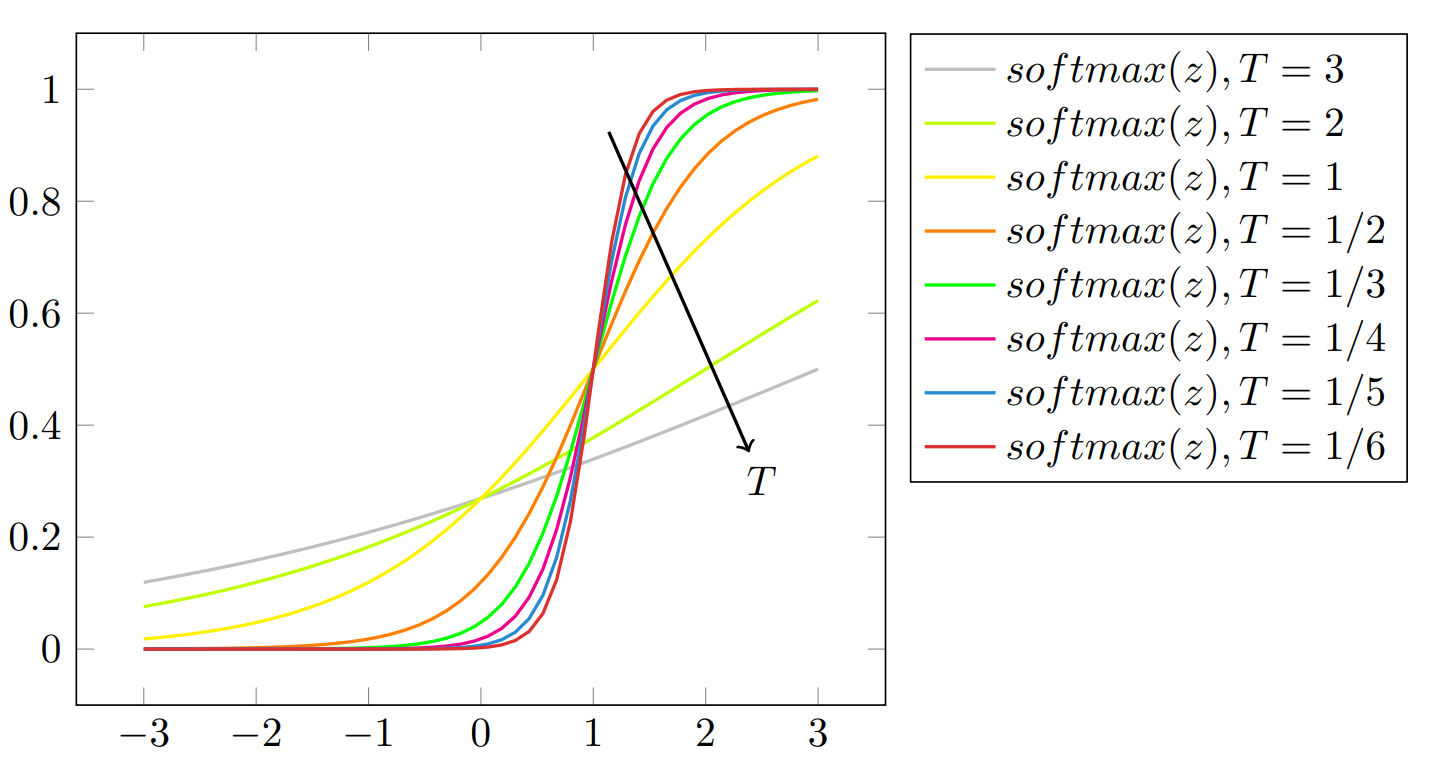
\includegraphics[width=\textwidth]{Figures/Softmaxbehaviour.png}
    \caption{The steepness of softmax function as temperature $T$ grows.}\label{fig:softmax}
\end{figure}

\section{Pooling}\label{sec:pooling}

In addition to discrete convolutions themselves, {\em pooling\/} operations
constitute another important building block in CNNs. Pooling operations reduce
the size of feature maps by using some function to summarize subregions, such
as taking the average or the maximum value.

Pooling works by sliding a window across the input and feeding the content of
the window to a {\em pooling function}. In some sense, pooling works very much
like a discrete convolution, but replaces the linear combination described by
the kernel with some other function. Fig. \ref{fig:numerical_average_pooling}
provides an example for average pooling, and Fig. \ref{fig:numerical_max_pooling}
does the same for max pooling.

The following properties affect the output size $o_j$ of a pooling layer
along axis $j$:

\begin{itemize}
    \item $i_j$: input size along axis $j$,
    \item $k_j$: pooling window size along axis $j$,
    \item $s_j$: stride (distance between two consecutive positions of the
        pooling window) along axis $j$.
\end{itemize}

\begin{figure}[p]
    \centering
    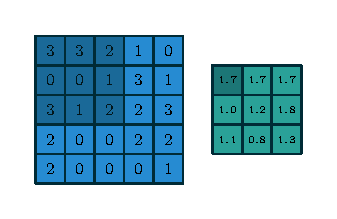
\includegraphics[width=0.32\textwidth]{pdf/numerical_average_pooling_00.pdf}
    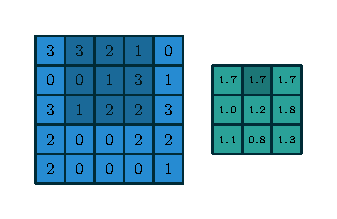
\includegraphics[width=0.32\textwidth]{pdf/numerical_average_pooling_01.pdf}
    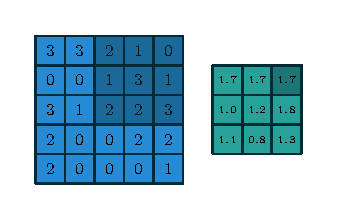
\includegraphics[width=0.32\textwidth]{pdf/numerical_average_pooling_02.pdf}
    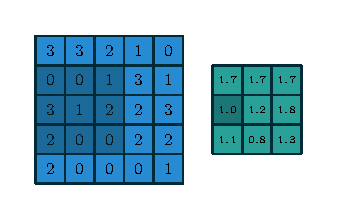
\includegraphics[width=0.32\textwidth]{pdf/numerical_average_pooling_03.pdf}
    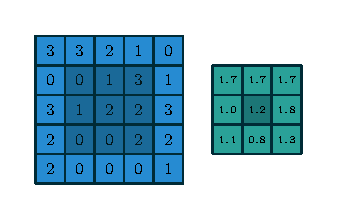
\includegraphics[width=0.32\textwidth]{pdf/numerical_average_pooling_04.pdf}
    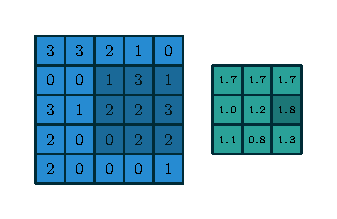
\includegraphics[width=0.32\textwidth]{pdf/numerical_average_pooling_05.pdf}
    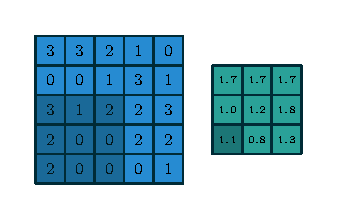
\includegraphics[width=0.32\textwidth]{pdf/numerical_average_pooling_06.pdf}
    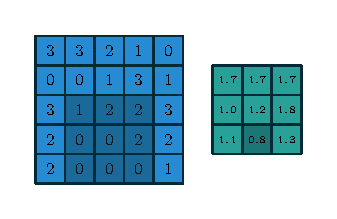
\includegraphics[width=0.32\textwidth]{pdf/numerical_average_pooling_07.pdf}
    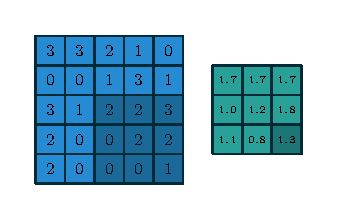
\includegraphics[width=0.32\textwidth]{pdf/numerical_average_pooling_08.pdf}
    \caption{\label{fig:numerical_average_pooling} Computing the output values
        of a $3 \times 3$ average pooling operation on a $5 \times 5$ input
        using $1 \times 1$ strides.}
\end{figure}

\begin{figure}[p]
    \centering
    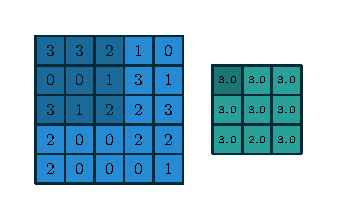
\includegraphics[width=0.32\textwidth]{pdf/numerical_max_pooling_00.pdf}
    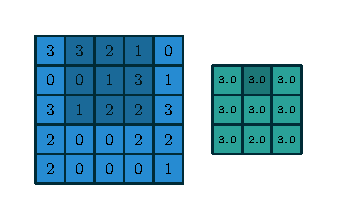
\includegraphics[width=0.32\textwidth]{pdf/numerical_max_pooling_01.pdf}
    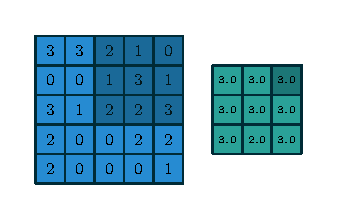
\includegraphics[width=0.32\textwidth]{pdf/numerical_max_pooling_02.pdf}
    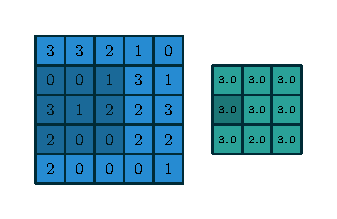
\includegraphics[width=0.32\textwidth]{pdf/numerical_max_pooling_03.pdf}
    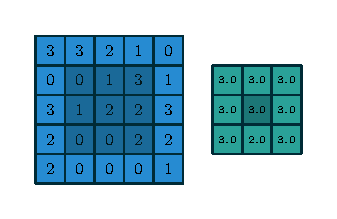
\includegraphics[width=0.32\textwidth]{pdf/numerical_max_pooling_04.pdf}
    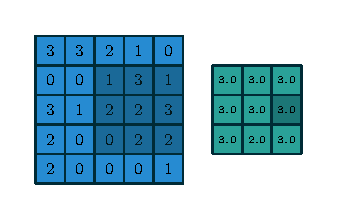
\includegraphics[width=0.32\textwidth]{pdf/numerical_max_pooling_05.pdf}
    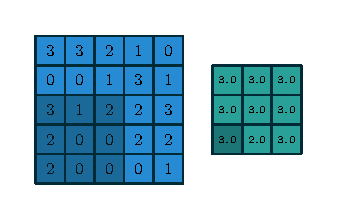
\includegraphics[width=0.32\textwidth]{pdf/numerical_max_pooling_06.pdf}
    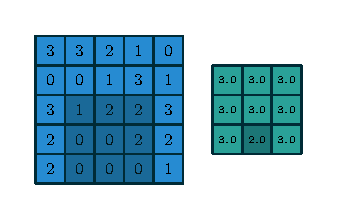
\includegraphics[width=0.32\textwidth]{pdf/numerical_max_pooling_07.pdf}
    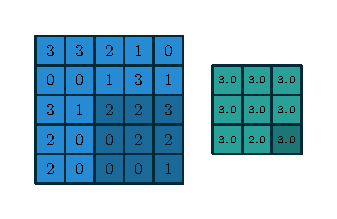
\includegraphics[width=0.32\textwidth]{pdf/numerical_max_pooling_08.pdf}
    \caption{\label{fig:numerical_max_pooling} Computing the output values of a
        $3 \times 3$ max pooling operation on a $5 \times 5$ input using $1
        \times 1$ strides.}
\end{figure}
